\documentclass[conference]{IEEEtran}
%\IEEEoverridecommandlockouts
% The preceding line is only needed to identify funding in the first footnote. If that is unneeded, please comment it out.
\usepackage[spanish]{babel}
\usepackage[utf8]{inputenc}
\usepackage{cite}
\usepackage{amsmath, amsthm,amssymb,amsfonts}
\usepackage{algorithmic}
\usepackage{graphicx}
\usepackage{textcomp}
\usepackage{xcolor}
\def\BibTeX{{\rm B\kern-.05em{\sc i\kern-.025em b}\kern-.08em
    T\kern-.1667em\lower.7ex\hbox{E}\kern-.125emX}}

% Definición del entorno 'definition'
\newtheorem{definition}{Definición}

\begin{document}

\title{Sistemas Lineales con Retardo: Predictores\\
	% {\footnotesize \textsuperscript{*}Note: Sub-titles are not captured in Xplore and
	% should not be used}
	% \thanks{Identify applicable funding agency here. If none, delete this.}
}

\author{
	\IEEEauthorblockN{José Alejandro León Sánchez}
	\IEEEauthorblockA{\textit{Posgrado de Ingeniería} \\
		\textit{UNAM}\\
		CDMX, Mexico}
	\and
	\IEEEauthorblockN{Basilio del Muro Cuellar}
	\IEEEauthorblockA{\textit{ESIME Culhuacán} \\
		\textit{IPN}\\
		CDMX, Mexico}
}

\maketitle

\begin{abstract}
	En esta ponencia, el Dr. Basilio Del Muro Cuéllar presentó una introducción detallada al problema de los sistemas lineales con retardos, destacando su relevancia en diversos contextos, desde procesos químicos hasta comunicaciones a distancia. Los retardos, comúnmente conocidos como tiempos muertos, representan el intervalo de tiempo en que un sistema no reacciona a una entrada antes de comenzar a mostrar una respuesta. Aunque a veces es posible despreciar estos retardos, existen muchos sistemas en los que su influencia es crucial. El Dr. Del Muro explicó, a manera intuitiva, la relación entre el integrador en los sistemas dinámicos y los retardos en sistemas discretos, y cómo estos dos elementos se combinan para formar el principal desafío que enfrentan los sistemas con retardos. La ponencia culminó con una discusión sobre estrategias de estabilización, predictores de Smith y Multipredictores para tratar sistemas inestables.
\end{abstract}

\begin{IEEEkeywords}
	Sistemas con retardos, tiempos muertos, estabilización, predictores, predictor de Smith, multipredictores.
\end{IEEEkeywords}

\section{Introducción}

Los retardos temporales, o tiempos muertos, son un fenómeno común en muchos sistemas físicos y de ingeniería. Un retardo puede entenderse como el lapso de tiempo durante el cual un sistema no responde inmediatamente a una señal de entrada, generando una respuesta solo después de que ha transcurrido un cierto tiempo. Este tipo de comportamiento es inevitable en sistemas como los procesos químicos, donde los retardos de transporte son críticos, así como en sistemas de comunicaciones y redes distribuidas, donde los retardos en la transmisión de datos pueden comprometer la estabilidad y el rendimiento global.

En sistemas dinámicos lineales, la presencia de un retardo puede afectar drásticamente la estabilidad del sistema. En sistemas continuos, las dinámicas están dominadas por integradores, mientras que en sistemas discretos el retardo unitario desempeña un papel equivalente. Cuando ambos fenómenos se combinan, la complejidad del análisis aumenta significativamente. El estudio de los sistemas con retardos busca no solo modelar estas dinámicas sino también desarrollar estrategias que aseguren la estabilidad y el rendimiento a pesar de los desafíos impuestos por los retardos.

Se exploraron diferentes enfoques para la estabilización de estos sistemas, comenzando con soluciones conservadoras aplicables a casos simples y evolucionando hacia técnicas más robustas que permiten lidiar con sistemas inestables. Se hace especial énfasis en los predictores, como el predictor de Smith y sus extensiones multipredictoras, que proporcionan soluciones eficaces para compensar el efecto de los retardos y mejorar el desempeño del sistema.


\section{Predictor de Smith}

El \textit{Predictor de Smith} es una técnica clásica de control diseñada para mejorar el rendimiento de sistemas lineales con retardos, eliminando el impacto negativo que estos tienen sobre el control. La idea principal es compensar el efecto del retardo temporal mediante la creación de un modelo interno de la planta sin retardo, separando así las dinámicas de la planta y el retardo. Este modelo anticipa la salida de la planta y permite que el controlador funcione como si el sistema no tuviera retardo.

Matemáticamente, el sistema con retardo se modela como:

\[
	y(t) = G(s) e^{-Ls} u(t),
\]

donde \( G(s) \) es la función de transferencia de la planta sin retardo, \( e^{-Ls} \) representa el retardo de tiempo \( L \), y \( u(t) \) es la entrada al sistema. El modelo interno utilizado por el \textit{Predictor de Smith} genera una estimación de \( y(t) \), anticipando la salida futura de la planta sin tener en cuenta el retardo (Figura \ref{fig:smith_predictor}).

\begin{figure}[htbp]
	\centerline{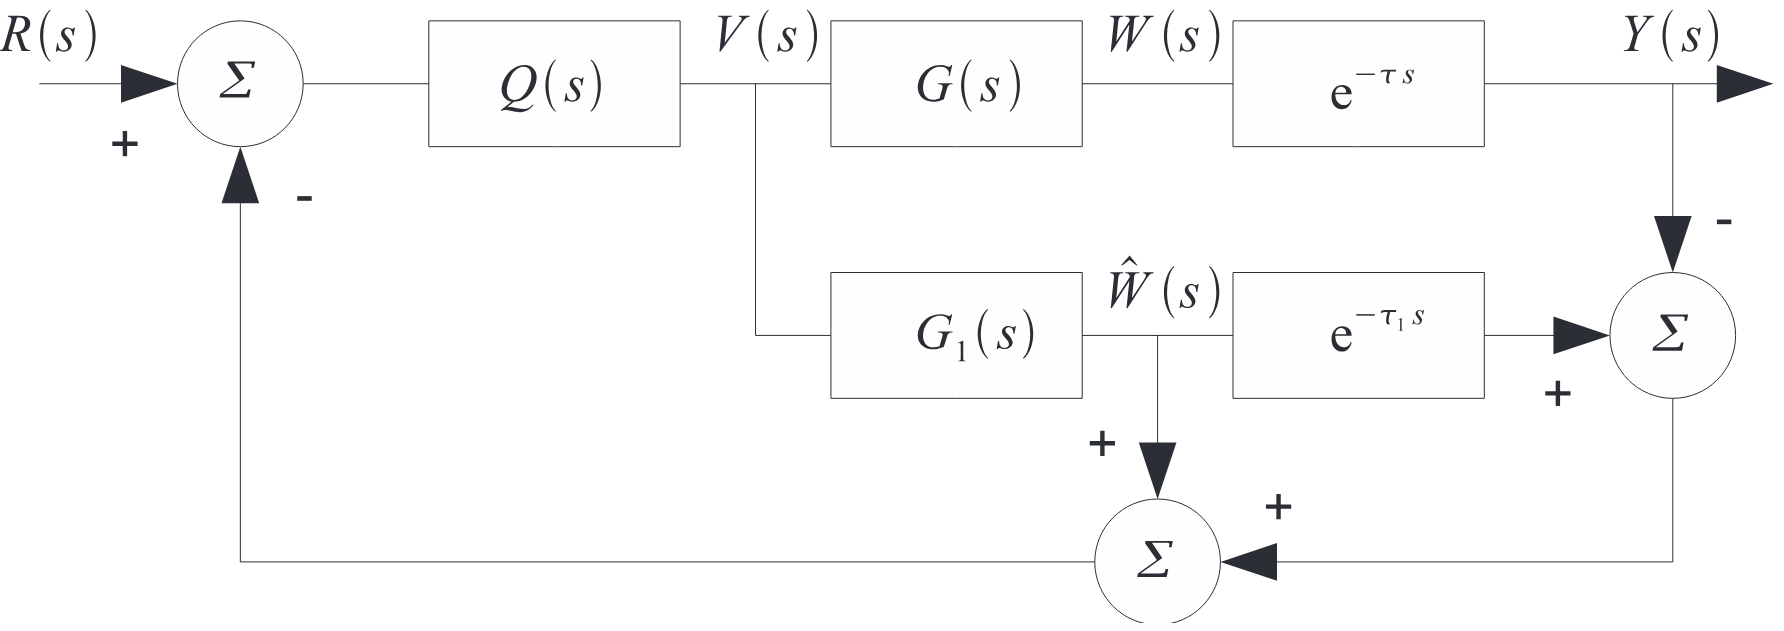
\includegraphics[width=0.5\textwidth]{smith_predictor.png}}
	\caption{Estructura del \textit{Predictor de Smith}.}
	\label{fig:smith_predictor}
\end{figure}

\subsection{Restricciones y características clave}

El \textit{Predictor de Smith} se caracteriza por ser un observador en lazo abierto, lo que significa que la estimación de la salida no se corrige en función de la salida real del sistema, sino que se basa únicamente en el modelo interno de la planta. Esto impone una limitación importante, ya que la precisión del modelo es crucial para garantizar un buen rendimiento del controlador.

Además, esta técnica está restringida principalmente a sistemas estables. Si el sistema tiene polos inestables, el \textit{Predictor de Smith} puede fallar en proporcionar una estabilización efectiva, ya que los polos inestables no pueden ser manejados de manera adecuada por un observador en lazo abierto. Es por ello que, en su forma original, el \textit{Predictor de Smith} se aplica típicamente a plantas con dinámica estable y tiempos muertos moderados.

\subsection{Compensación Predictiva para Sistemas con Retardo}

El predictor de Smith modifica la dinámica del sistema mediante la estimación del estado futuro en función del retardo temporal. Este enfoque resulta efectivo cuando el retardo es conocido y el sistema subyacente es estable. Sin embargo, para mejorar la robustez en sistemas con retardos mayores, se han propuesto modificaciones adicionales que amplían su aplicabilidad.

Una de estas extensiones, inspirada por trabajos de Michiels et. al.\cite{michiels2002continuous} y presentada en los resultados, divide el retardo total en dos fracciones \(\tau_1 = \frac{\tau}{3}\) y \(\tau_2 = \frac{2\tau}{3}\), permitiendo mejorar el límite del retardo que puede ser compensado. Mientras que los controladores tradicionales \(P\) o \(PI\) requieren que \(\tau < \frac{1}{a} - \sum\frac{1}{b_i}\), el esquema predictivo propuesto extiende este límite a \(\tau < \frac{3}{a}\). Esto desplaza los polos inestables hacia el semiplano izquierdo, mejorando la estabilidad general del sistema ante retardos más significativos.

Este enfoque proporciona una solución más eficiente para la compensación de retardos en sistemas inestables, permitiendo así una mayor robustez en sistemas sujetos a perturbaciones y tiempos muertos.



\section{Conclusiones}
La inclusión de retardos en sistemas lineales es un aspecto crítico que debe ser considerado en el diseño de estrategias de control. Los retardos no solo complican el análisis de la estabilidad, sino que también pueden comprometer el rendimiento del sistema. El uso de predictores, como el predictor de Smith, representa una herramienta valiosa para mitigar estos efectos, permitiendo que los controladores operen de manera más efectiva a pesar de la presencia de retardos.

Además, la exploración de técnicas avanzadas, como la división del retardo en fracciones para mejorar la robustez del sistema, subraya la importancia de la adaptabilidad en el diseño de controladores.

\begin{thebibliography}{00}
	\bibitem{michiels2002continuous}
	Michiels, W., Engelborghs, K., Vansevnant, P., \& Roose, D. (2002). Continuous pole placement for delay equations. *Automatica*, 38(5), 747–761.
	\bibitem{delmuro2012unstable}
	Del Muro-Cuéllar, B., Márquez-Rubio, J. F., Velasco-Villa, M., \& Álvarez-Ramírez, J. J. (2012). On the control of unstable first order linear systems with large time lag: Observer based approach. *European Journal of Control*, 18(5), 439–451. Elsevier.
	\bibitem{HERNANDEZPEREZ202098}
	M.A. Hernández–Pérez, V. Fragoso–Rubio, M. Velasco–Villa, B. del Muro–Cuéllar, J.F. Márquez–Rubio, H. Puebla, "Prediction-based control for a class of unstable time-delayed processes by using a modified sequential predictor," \textit{Journal of Process Control}, vol. 92, pp. 98-107, 2020.
\end{thebibliography}

\end{document}
